\documentclass{beamer}
\usepackage{graphicx}
\usepackage{PaloAlto}
\usepackage{tikz-cd}
\usecolortheme{sidebartab}
\usepackage{latexsym,amsmath,amssymb}

\title{Turing award winner}
\subtitle{Raj Reddy :The  $ 28^{th} $ Turing awardee}
\author{P.Anurag}
\institute{SCIS University of Hyderabad}
\date{\today}

%\setbeamertemplate{frametitle continuation}{\gdef\beamer@frametitle{}}
\usebackgroundtemplate{%
\tikz\node[opacity=0.35] {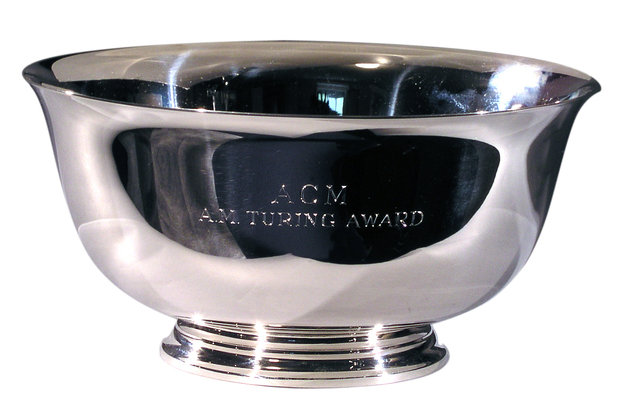
\includegraphics[height=0.955\paperheight,width=\paperwidth]{turing_bowl.jpg}};}

\begin{document}
 
  \usebackgroundtemplate{%
\tikz\node[opacity=0.35] {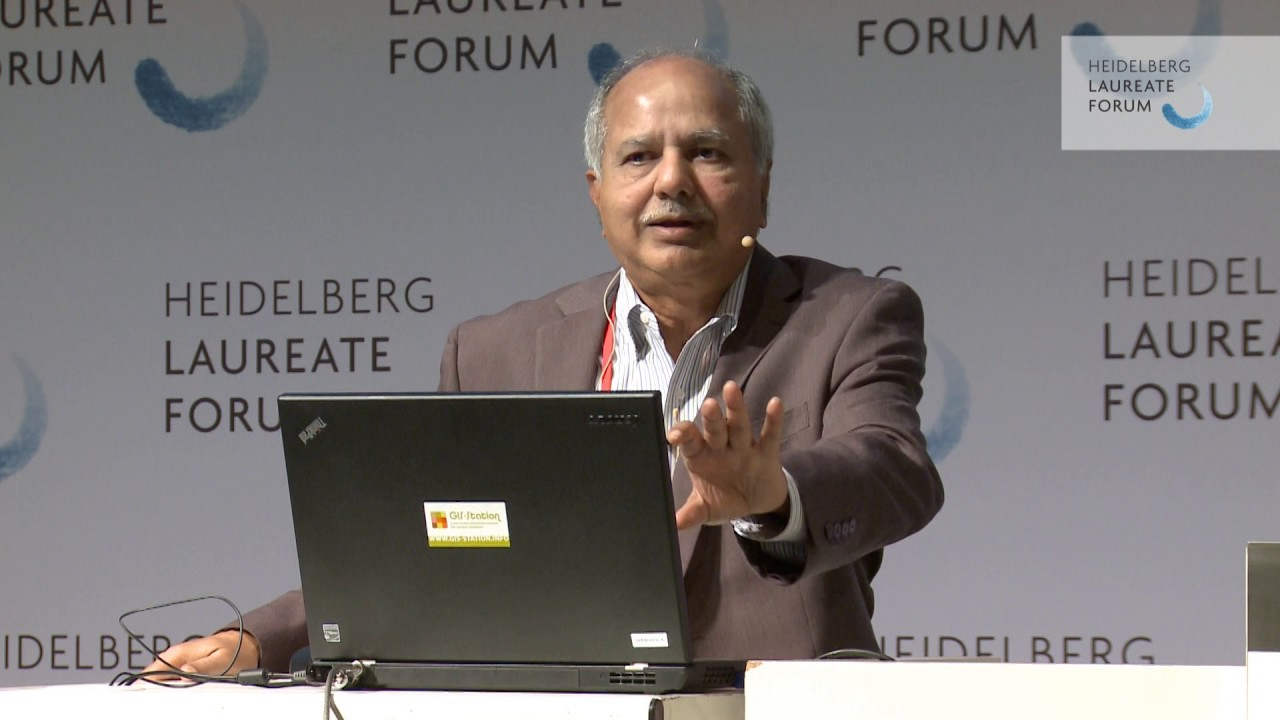
\includegraphics[height=0.95\paperheight,width=\paperwidth]{raj123.jpg}};}
\maketitle
 
\begin{frame}
\begin{figure}
 \centering
 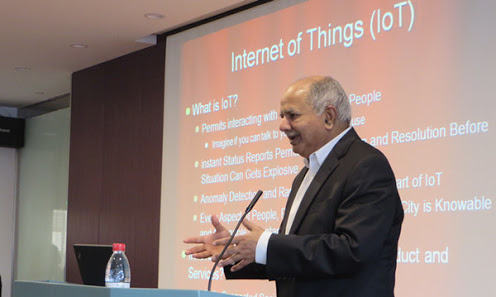
\includegraphics[scale=0.5]{raj1.jpg}
\end{figure} 

\begin{block}{}
 Raj Reddy  Moza Bint Nasser Professor of Computer science and Robotics at 
 Carnegie Mellon University$^{\tiny \cite{1}}$.
\end{block}
\end{frame}

\begin{frame}
  \frametitle{Table of contents}
  \tableofcontents
\end{frame}

\begin{frame}
 \section{Introduction}
 \transdissolve
 \frametitle{Introduction}
 \begin{block}{}
   Dabbala Rajagopal Reddy
 \end{block}

 \begin{columns}
  \begin{column}{0.35\textwidth}
   \begin{center}
     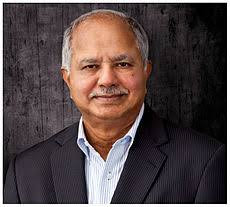
\includegraphics[scale=0.5]{raj.jpeg} \\
     Raj Reddy
   \end{center} 
   \end{column}
   %
   
  \begin{column}{0.55\textwidth}
   \begin{block}{\bf Introduction}  
    {\bf Dabbala Rajagopal "Raj" Reddy} is an Indian-American computer 
    scientist and a winner of the Turing Award.He is also the chairman 
    of International Institute of Information Technology, Hyderabad.
    \end{block}
  \end{column}
 \end{columns}
\end{frame}

 \section{Early Life}
\begin{frame}
 \transblindshorizontal
  \frametitle{\bf Early Life}
 \setbeamercovered{transparent}
  \begin{itemize}
   \item<1-> Dabbala Rajagopal Reddy was born on 13 June 1937 in Katur, Chitoor
   district,Madras Presidency, British Raj.
   \item<2-> His father, Sreenivasulu, was an agricultural landlord.
   \item<3-> His mother, Pitchamma, was a homemaker
  \end{itemize} 
\end{frame}
{\gdef\beamer@frametitle{}}
 
 \section{Qualifications}
\begin{frame}[t]
 \frametitle{\bf Qualifications}
 \transboxin
  \begin{block}{}
   \begin{table}
    \begin{tabular}{cccc}
     \uncover<1->{{\bf Degree} & {\bf Specilization} & {\bf Year} & {\bf institute} \\}
     \uncover<2->{\begin{tabular}{@{}c@{}}
                   Bachelor of \\ Technology
                  \end{tabular} & Civil engneering & 1958 &
                           \begin{tabular}{@{}c@{}}
                            University of  \\ Madras \\ (now {\bf Anna}\\{\bf University})
                           \end{tabular} \\}
     \uncover<3->{\begin{tabular}{@{}c@{}}
                    Master of \\ Technology
                  \end{tabular} & Information  Technology & 1960 & 
                                                   \begin{tabular}{@{}c@{}}
                                                     University of\\new south\\wales
                                                   \end{tabular} \\}
  
     \uncover<4->{Doctorate & Computer   Science & 1966 & \begin{tabular}{@{}c@{}}
                                                           Stanford  \\ university
                                                         \end{tabular}}
    \end{tabular}
   \end{table}
  \end{block}
\end{frame}

 \section{Career}
  \usebackgroundtemplate{%
\tikz\node[opacity=0.35] {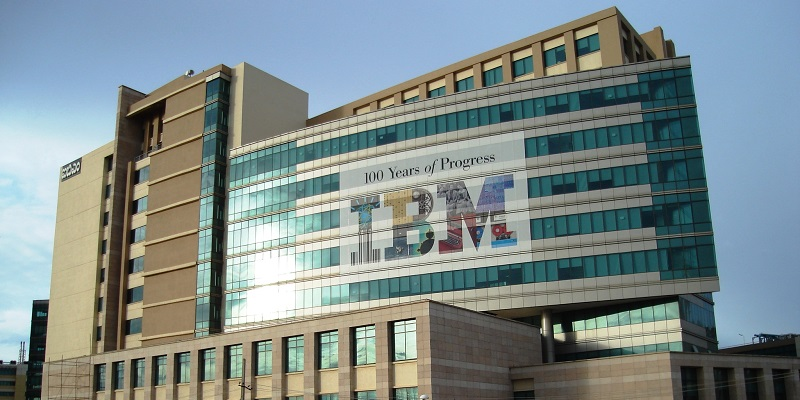
\includegraphics[height=\paperheight,width=\paperwidth]{raj1ibm.jpg}};}
\begin{frame}%[allowframebreaks]
 \transblindsvertical
 \frametitle{Career}
   \setbeamercovered{dynamic}
 \begin{columns}
  \begin{column}{0.19\textwidth}
    
  \onslide<1->{ \begin{block}{}
    1960-63
   \end{block}}
   
\end{column}

  \begin{column}{0.7\textwidth}
  \onslide<2->{\begin{block}{}
               Applied Science Representative for IBM Corp. in Australia$^{\tiny\cite{2}}$.
               \end{block}}
  \end{column}
 \end{columns}
 
 \begin{center}
  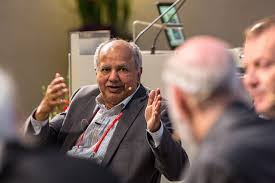
\includegraphics[scale=0.5]{rajibm.jpeg}
 \end{center}
 
\end{frame}

 \usebackgroundtemplate{%
\tikz\node[opacity=0.35] {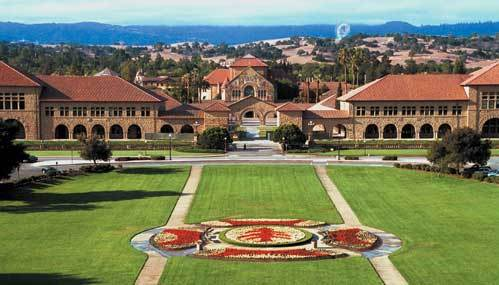
\includegraphics[height=\paperheight,width=\paperwidth]{raj1stanford.jpg}};}
\begin{frame}
 \transblindsvertical
  \frametitle{Career}
   \setbeamercovered{dynamic}
 
  \begin{columns}
  \begin{column}{0.19\textwidth}
      \onslide<1->{\begin{block}{}
		    1966-69
		   \end{block}}
  \end{column}
  
  \begin{column}{0.7\textwidth}
     \onslide<2->{\begin{block}{}
		Assistant Professor of Computer Science at Stanford.
	       \end{block}}
  \end{column}
  \end{columns}
  
  \begin{center}
   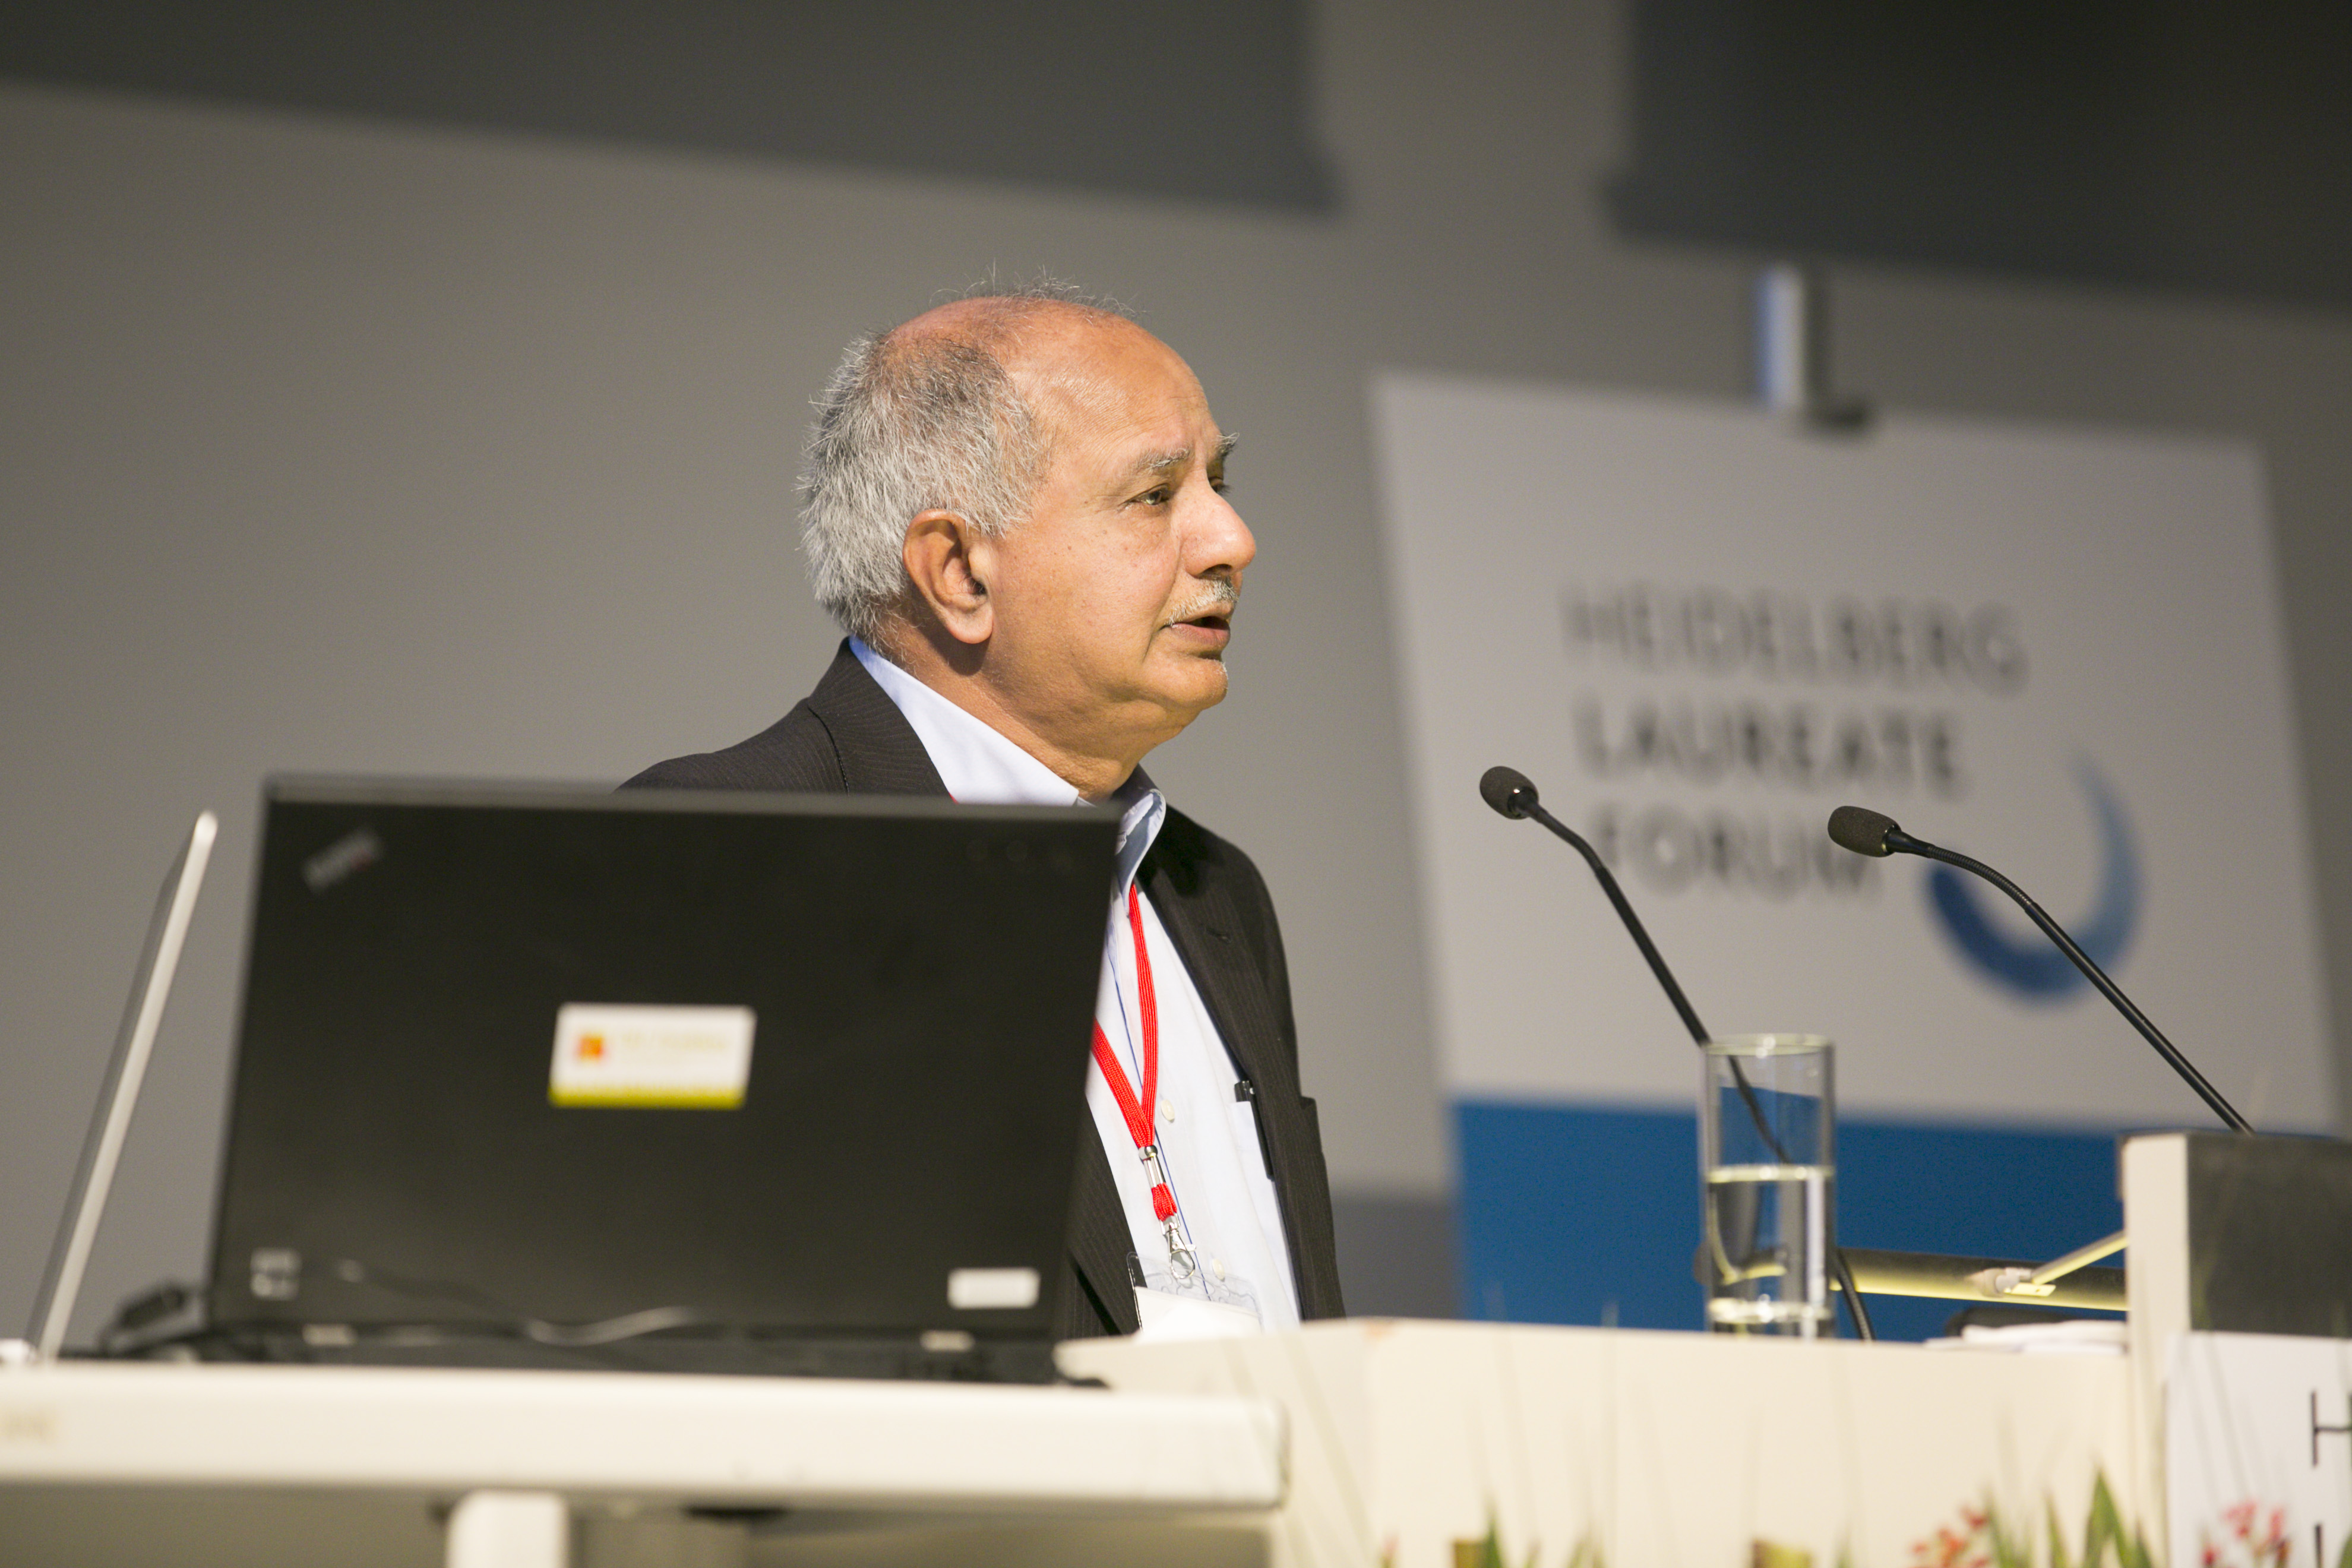
\includegraphics[scale=0.15]{rajstanford.jpg}
  \end{center}

\end{frame}

 \usebackgroundtemplate{%
\tikz\node[opacity=0.35] {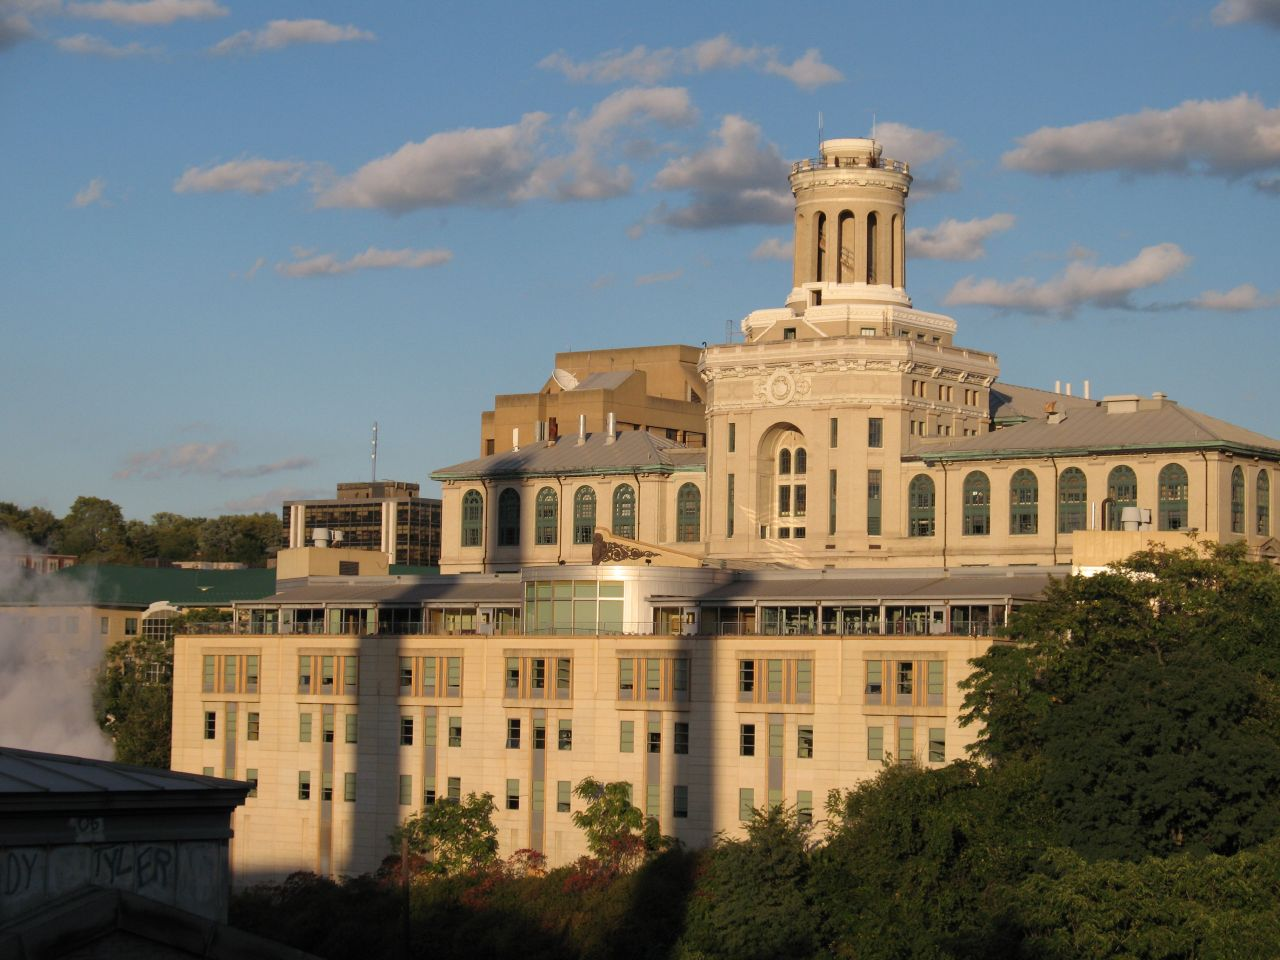
\includegraphics[height=\paperheight,width=\paperwidth]{raj1cmu.jpg}};}
\begin{frame}
  \transblindsvertical
  \frametitle{Career}
   \setbeamercovered{dynamic}
   
    \begin{columns}
  \begin{column}{0.1\textwidth}
    

   \onslide<1->{\begin{block}{}
    1969
   \end{block}}
   
  \onslide<3->{\begin{block}{}
    1973
   \end{block}}
   
  \onslide<5->{\begin{block}{}
    1984
   \end{block}}
  
  \end{column}
 
  \begin{column}{0.6\textwidth}

  \onslide<2->{\begin{block}{}
		Carnegie Mellon Faculty as an Associate Professor of Computer Science.
	       \end{block}}
 
  \onslide<4->{\begin{block}{}
                Carnegie Mellon Faculty as a Full-time Professor of Computer Science.
	        \end{block}}
 
  \onslide<6->{\begin{block}{}
		Carnegie Mellon Faculty as an University Professor of Computer Science.
	        \end{block}}

  \end{column}
  
 \end{columns}
\end{frame}


\usebackgroundtemplate{%
\tikz\node[opacity=0.35] {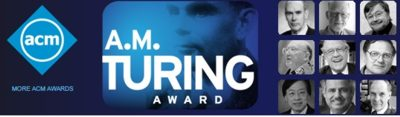
\includegraphics[height=\paperheight,width=\paperwidth]{turing.jpg}};}
 \section{Awards and Honours}
\begin{frame}[allowframebreaks]
 \frametitle{Awards and Honours}
 
  {\bf Legion of Honor:}
    \begin{center}
     
\includegraphics[scale=0.35]{rajloh.png}
    \end{center}
    
    In 1984, Reddy was awarded the French Legion of Honour 
    by the French President Fran\c{c}ois Mitterrand.        
     \framebreak
              
    {\bf Turing award:} 
    \begin{columns}
     \begin{column}{0.45\textwidth}
      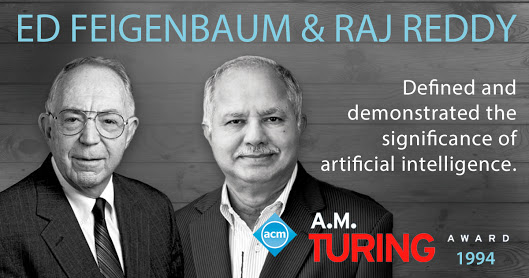
\includegraphics[scale=0.2615]{rajco.jpg}
     \end{column}
     
     \begin{column}{0.45\textwidth}
     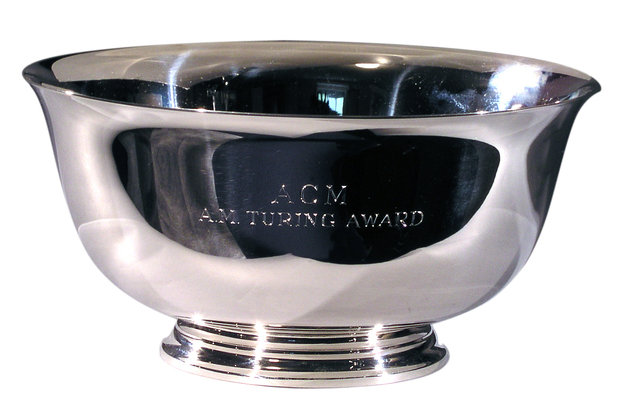
\includegraphics[scale=0.2125]{turing_bowl.jpg}
     \end{column}
    \end{columns} 
    
     In 1994, he and Edward Feigenbaum received the ACM Turing Award$^{\tiny\cite{7}}$.
     \framebreak
     
    {\bf Padma Bhushan:}
    \begin{columns}
     \begin{column}{0.5\textwidth}
      \begin{center}
       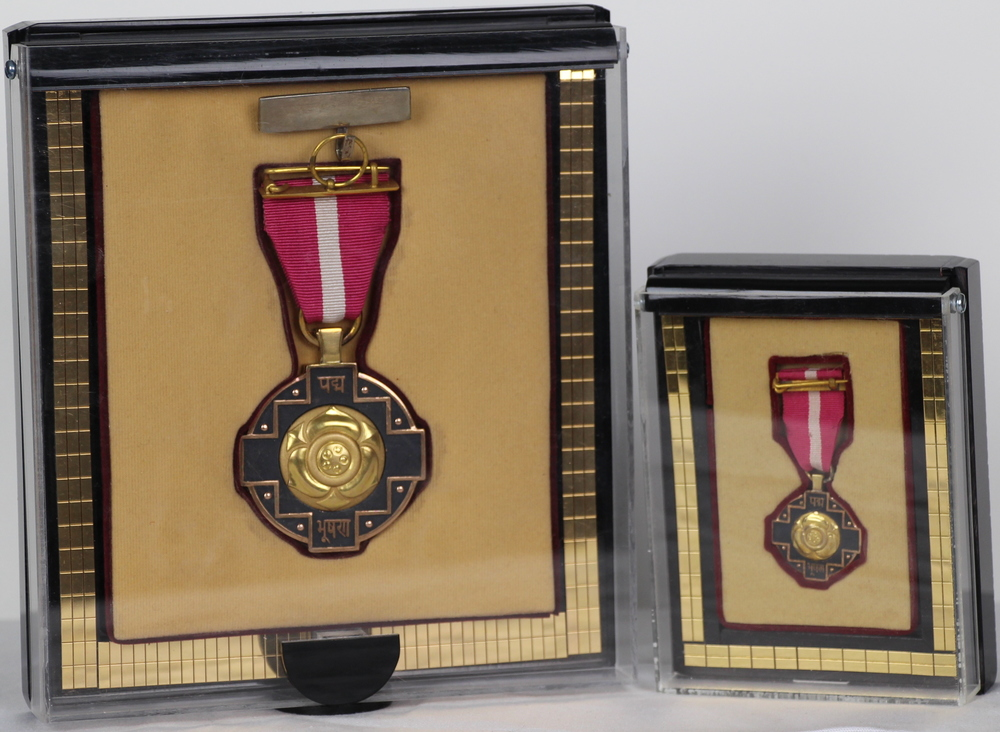
\includegraphics[scale=0.13]{rajpb.JPG}
      \end{center}
      \end{column}
      
      \begin{column}{0.5\textwidth}
       \begin{center}
        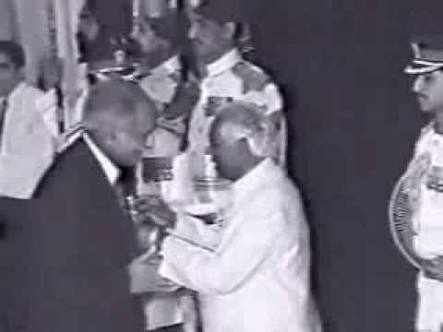
\includegraphics[scale=0.3]{pb.jpg}
       \end{center}

      \end{column}

    \end{columns}
    
      In 2001, Reddy was awarded Padma Bhushan$^{\tiny\cite{8}}$, an award given by Indian
      government.
                      
\end{frame}
%\framebreak
 
\begin{frame}
 \frametitle{Awards and Honours IV}
 \setbeamercovered{dynamic}
 
  \onslide<1>\begin{block}{}
      	      In 2006, he received the Vannevar Bush Award. 
	      \end{block}
 
  \onslide<2>\begin{block}{}
	      In 2008, Reddy received the IEEE James L.Flanagan Speech and Audio 
	      Processing Award. 
	     \end{block}   
     \begin{figure}
      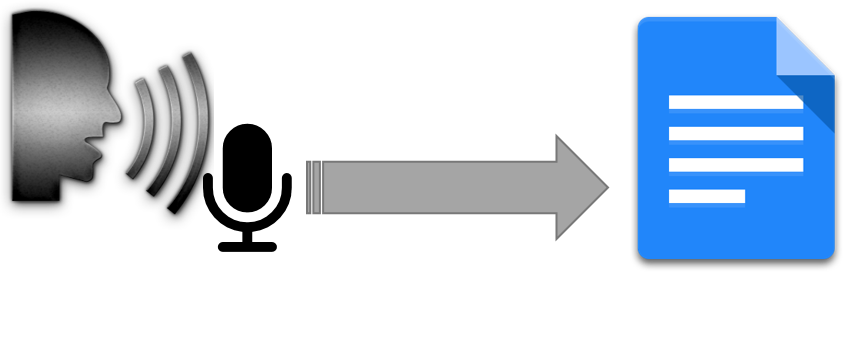
\includegraphics[scale=0.5]{rajsrs.png}
      \caption{Sphinx Speech Recognition}
     \end{figure}

\end{frame}

 \section{Contributions}
\begin{frame}
\transwipe
 \frametitle{Contributions}
 \begin{itemize}
  \item Machine Intelligence and Robotics: Report of the NASA Study Group 
   Executive Summary$^{\tiny\cite{10}}$.
  \item Foundations and Grand Challenges of Artificial Intelligence, AAAI 
   Presidential Address, 1988$^{\tiny\cite{9}}$.
  \item To Dream the Possible Dream, Turing Award Lecture presented at ACM
   CS Conference, March 1, 1995.
 \end{itemize}
\end{frame}
 
\section{Fields of Interest}
\begin{frame}
 \transwipe
 \frametitle{Fields of Interest} 
 \begin{columns}
  \begin{column}{0.35\textwidth}
    \only<2>{\begin{block}{}
     Artificial Intelligence
    \end{block}}
    
   \only<3>{\begin{block}{}
     Robotics
    \end{block}}
    
    \only<4>{\begin{block}{}
     Human-Computer Interaction
    \end{block}}
  \end{column}

  \begin{column}{0.5\textwidth}
   
    \only<2>{\begin{center}
     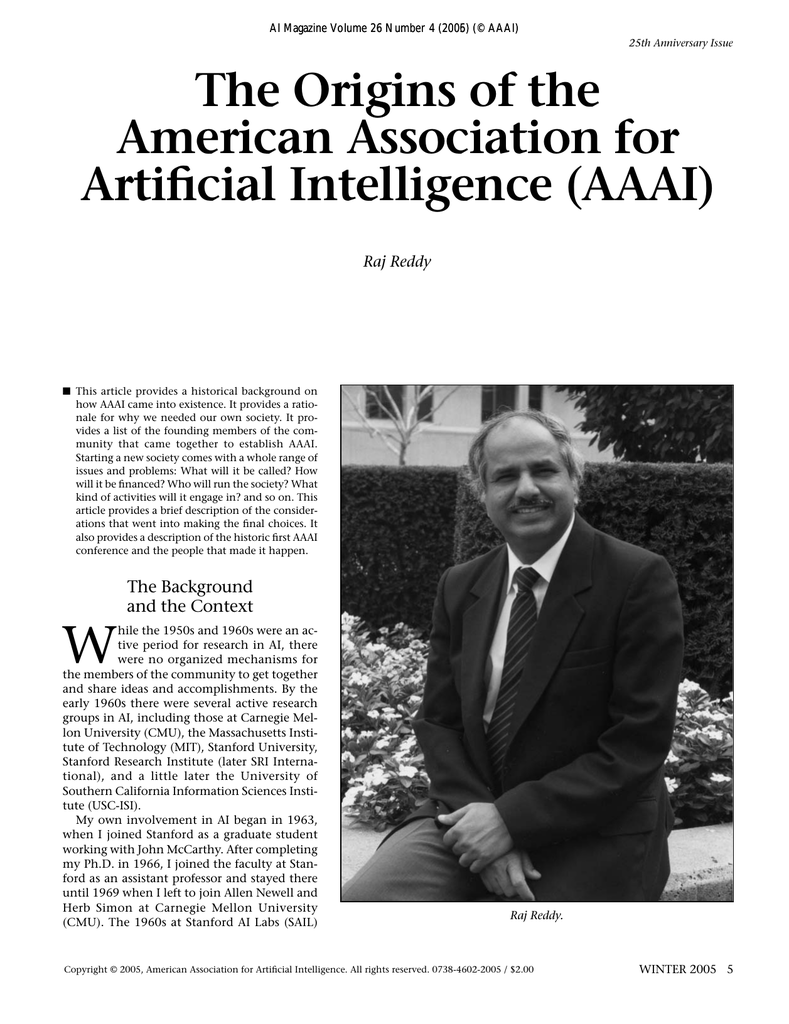
\includegraphics[scale=0.35]{airaj.png}
    \end{center}}
    
    \only<3>{\begin{center}
     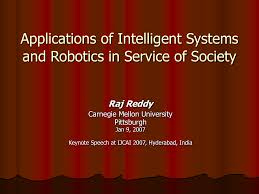
\includegraphics[scale=0.55]{robo1.jpeg}
    \end{center}}
    
    \only<4>{\begin{center}
     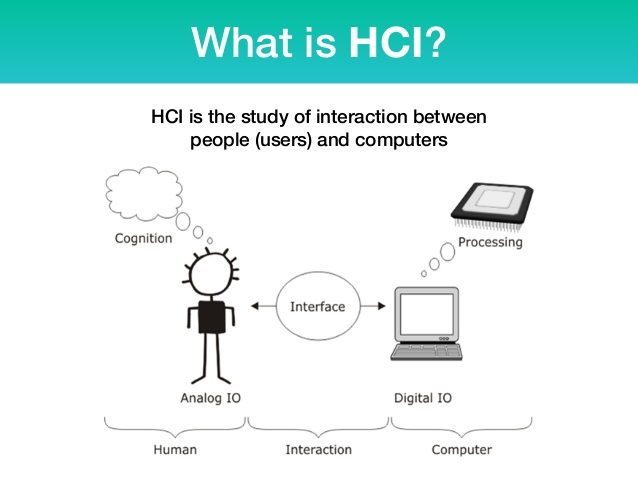
\includegraphics[scale=0.25]{hci-basics-2-638.jpg}
    \end{center}}

  \end{column}
 \end{columns}
\end{frame}

 \usebackgroundtemplate{%
\tikz\node[opacity=0.35] {
\includegraphics[height=\paperheight,width=\paperwidth]{rajtq2.jpeg}};}
\section{References}
\begin{frame}[allowframebreaks]
 \frametitle{References}
 \begin{thebibliography}{}
  \bibitem{1}
  \url {https://en.wikipedia.org/wiki/Raj_Reddy}
  \bibitem{2}
  \url {www.rr.cs.cmu.edu/}
  \bibitem{3}
  \url {amturing.acm.org/award_winners/reddy_9634208.cfm}
  \bibitem{4}
  \url {scientistsinformation.blogspot.com/2010/02/professor-raj-reddy.html}
  \bibitem{5}
  \url {https://www.britannica.com/biography/Raj-Reddy}
  \bibitem{6}
  "NNDB Listing". NNDB. Retrieved August 26, 2011.
  \bibitem{7}
   "ACM Award Citation / Raj Reddy".\url{awards.acm.org}. Retrieved July 25, 2011.
   \framebreak   
  \bibitem{8}
    "Padma Bhushan Awardees — Padma Awards".\url{india.gov.in}. Retrieved July 25, 2011.
  \bibitem{9}
   "Foundations and Grand Challenges of Artificial Intelligence". AAAI Magazine. 9 (4): 9–21.
  \bibitem{10}
  Machine Intelligence and Robotics Executive Summary. Carnegie Mellon University. Retrieved September 7, 2011.
  \bibitem{11}
  Machine Intelligence and Robotics: Report of the NASA Study Group. Carnegie
  Mellon University. Retrieved September 7, 2011.
  \bibitem{12}
   "Honda Prize 2005". Honda Foundation. Retrieved August 3, 2011.
 \end{thebibliography}

\end{frame}

\end{document}